\documentclass{protokoll}
\usepackage{booktabs,multirow,xspace}
\newcommand{\assistent}{C. Lenk}
\newcommand{\versuch}{Mottstreuung}
\newcommand{\nummer}{P527}

\newcommand{\Isotop}[2]{\ensuremath{^{#2}\mathrm{#1}}\xspace}
\newcommand{\FWHM}{E^\mathrm{FWHM}}

\begin{document}

\section{Einleitung}


\section{Theoretische Grundlagen}
\subsection{$\beta$-Zerfall}
\label{cha:beta}
Der $\beta$-Zerfall subsummiert drei Zerf�lle, bei denen sich $Z$ um eins �ndert, $A$ jedoch konstant bleibt. 
\begin{description}
\item[$\beta^-$-Zerfall:] Beim $\beta^-$-Zerfall zerf�llt ein Neutron innerhalb des Kerns in ein Proton, ein Elektron sowie ein Anti-Elektronneutrino:
    \begin{align}
      n \to p + e^- + \bar\nu_e
    \end{align}
    Dieser Zerfall ist bei $m(A,Z) > m(A,Z+1)$ energetisch m�glich.

\item[$\beta^+$-Zerfall:] Beim $\beta^+$-Zerfall hingegen zerf�llt ein gebundenes Proton in ein Neutron, ein Positron und ein Elektronneutrino:
    \begin{align}
      p \to n + e^+ + \nu_e
    \end{align}
    Dieser Zerfall ist bei $m(A,Z) > m(A,Z-1) + 2 m_e$ energetisch m�glich.

\item[Elektroneneinfang:] Des Weiteren existiert noch die M�glichkeit des
    Elektroneneinfangs. Da die Elektronen im Atom eine endliche
    Aufenthaltswahrscheinlichkeit im Kern haben, k�nnen diese Elektronen von einem
    Proton eingefangen werden. Hierbei entsteht ein Neutron und ein Elektronneutrino:
    \begin{align}
      p + e^- \to n + \nu_e
    \end{align}
    Dieser Zerfall ist bei $m(A,Z) > m(A,Z-1) + E^{e^-}_{\text{Bind}}$
    energetisch m�glich, wobei $E^{e^-}_{\text{Bind}}$ die Bindungsenergie des
    Elektrons darstellt. In der jeweiligen Elektronenschale wird eine L�cke
    hinterlassen. Der Atomkern ist nun angeregt.

%noch nicht fertig
 
\subsection{Parit�t}

\subsection{Spinpolarisation}

\subsection{Mottstreuung}

\subsection{Messgr��en}

\subsection{Szintillationsdetektor}
Ein Szintillationsdetektor besteht aus zwei Teilen, einem Szintillator und einem
Photomultiplier (siehe Abb. \ref{fig:szinti}). Im Szintillator erzeugen die
nachzuweisenden Teilchen (hier Elektronen) einen Lichtblitz (Lumineszenzlicht),
welches vom Photomultiplier (siehe Abschnitt \ref{cha:photo}) in ein
elektrisches Signal umgewandelt wird. Als Szintillatormaterial werden
anorganische Einkristalle wie NaI, organische Fl�ssigkeiten und organisches
Plastikmaterial (wie in diesem Versuch) oder Edelgase verwendet.

\begin{figure}[H]
  \centering
  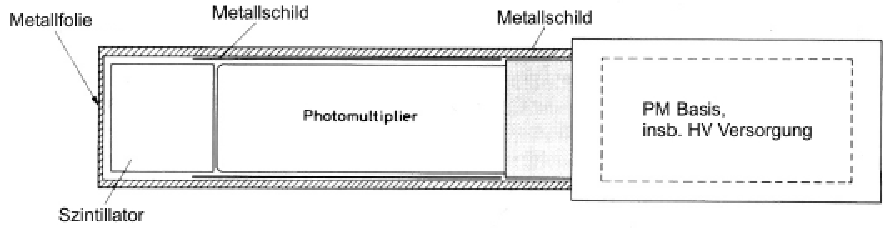
\includegraphics[width=0.55\textwidth]{grafiken/szinti}
  \caption[Szintillationsdetektor]{Schematischer Aufbau eines
  Szintillationsdetektors~\cite{leo}}
  \label{fig:szinti}
\end{figure}

% Plastikszintillator!
Je nach Verwendungszweck wird der Szintillator ausgew�hlt. Im vorliegenden Fall
ergeben sich die Szintillationsmechanismen aus den im B�ndermodell (siehe
Abschnitt \ref{cha:halb}) offensichtlich werdenden Eigenschaften des
anorganischen Kristalls. Das einfallende Teilchen wird entweder ein Elektron vom
Valenz- ins Leitungsband heben, wobei auch ein Loch im Valenzband entsteht, oder
es wird ein sogenanntes Exciton erzeugen. Dieses ist ein direkt unter das
Leitungsband angeregtes Elektron (in Abb. \ref{fig:szinti2} als Excitonband
bezeichnet). Elektron und Loch bleiben, wie in der Abbildung auch angedeutet,
dabei jedoch aneinander gebunden und bewegen sich so, ohne zum Ladungstransport
im Kristall beizutragen, frei durch selbigen. Unter der Emission eines Photons
der Bandl�ckenenergie k�nnen diese Elektron-Loch-Paare anschlie�end wieder
rekombinieren. Da somit nat�rlich die Energie der Photonen gerade der Bandl�cke
entspricht, w�rde eine sofortige Absorption durch den Kristall erfolgen, was
selbstverst�ndlich nicht gew�nscht ist. Deshalb dotiert man den Kristall mit
Fremdatomen und legt so energetisch erlaubte Zwischenzust�nde in der Bandl�cke
(verbotene Zone) an (siehe erneut Abb. \ref{fig:szinti2}). Bei der Rekombination
�ber ein solches Lumineszenszentrum erfolgt die Emission einiger
niederenergetischer Photonen. Diese k�nnen dann wegen der geringen
Dotierungsdichte ungehindert den Photomultiplier erreichen und detektiert
werden.

\begin{figure}[H]
  \centering
  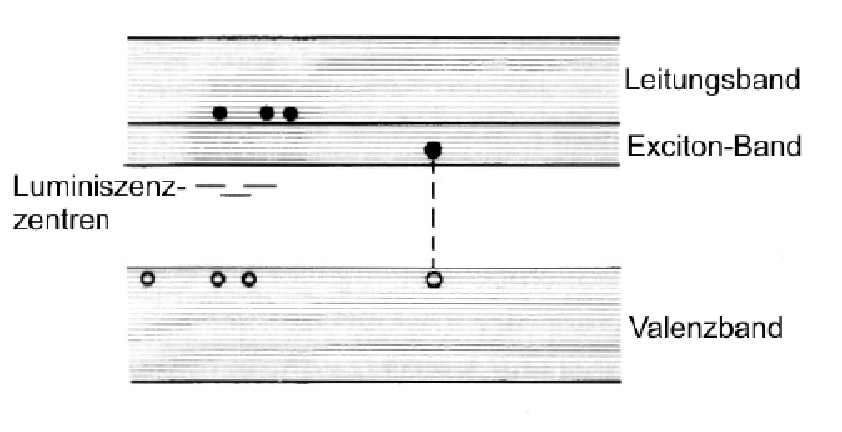
\includegraphics[width=0.55\textwidth]{grafiken/szinti2}
  \caption[Szintillationsdetektor]{Bandstruktur eines
  Szintillationsdetektors~\cite{leo}}
  \label{fig:szinti2}
\end{figure}

Die bei der Detektion von $\gamma$-Strahlung am Photomultiplier ankommenden
Lumineszenzblitze werden in selbigem in Ladung, also in messbare Spannungspulse
umgewandelt (siehe Abschnitt \ref{cha:photo}). Diese Pulse sind idealerweise
zeitlich und energetisch direkt mit den einfallenden Photonen korreliert. Die
zeitliche Aufl�sung des Detektors h�ngt somit vor allem vom zeitlichen Verlauf
des Lichtsignals des Szintillators und von der Laufzeit der Ladungstr�ger im
Photomultiplier ab. Eine typische Lichtkurve eines Szintillators ist in
Abbildung (\ref{fig:lichtkurve}) zu sehen.

\begin{figure}[H]
  \centering
  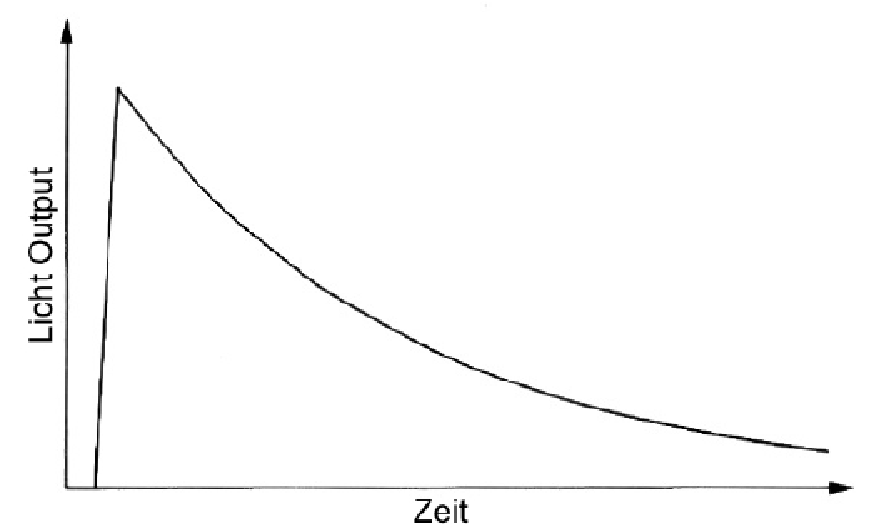
\includegraphics[width=0.35\textwidth]{grafiken/lichtkurve}
  \caption[Lichtkurve]{Lichtkurve eines Szintillators~\cite{leo}}
  \label{fig:lichtkurve}
\end{figure}

Zun�chst ist ein steiler Anstieg (Anstiegszeit liegt bei etwa
$\unit[10^{-10}]{s}$) zu beobachten. Die durch die Lebensdauer der angeregten
Zust�nde vorgegebene Abstiegszeit liegt bei etwa $\unit[(10^{-9} -
10^{-5})]{s}$.  Eine kurze Lebensdauer ist also ein Auswahlkriterium f�r ein
Szintillatormaterial, um die Zeitaufl�sung zu verbessern und die Totzeit zu
verk�rzen.

\subsubsection{Photomultiplier}
\label{cha:photo}
Ein Photomultiplier ist ein lichtsensitives Bauteil, welches einfallende
Photonen in einen messbaren elektrischen Strom umwandelt. Dies geschieht wie
folgt (siehe auch Abb.~\ref{fig:photo}). F�llt Strahlung auf die Photokathode
aus photosensitivem Material, so werden Elektronen �ber den photoelektrischen
Effekt emittiert. Hierbei werden Effizienzen von etwa $\unit[30]{\%}$ erreicht.
�ber ein angelegtes elektrisches Feld werden diese Elektronen nun auf die erste
Dynode hin beschleunigt. Dort werden pro einfallenden Elektrons bis zu zehn
Sekund�relektronen ausgeschlagen. Zwischen den einzelnen Dynoden, insgesamt gibt
es etwa zehn St�ck, liegen ebenfalls Spannungen an. Die Potentiale sind so
gew�hlt, dass die Elektronen stets allesamt zur n�chsten Dynode beschleunigt
werden, wo sie erneut Sekund�relektronen ausschlagen usw.. Auf diese Weise kann
eine Verst�rkung des Eingangssignals von etwa $10^6$ bis $10^7$ an der Anode
erreicht werden. Dabei ist die Amplitude des Ausgangssignals proportional zur
Energie des einfallenden Photons.

\begin{figure}[h]
  \centering
  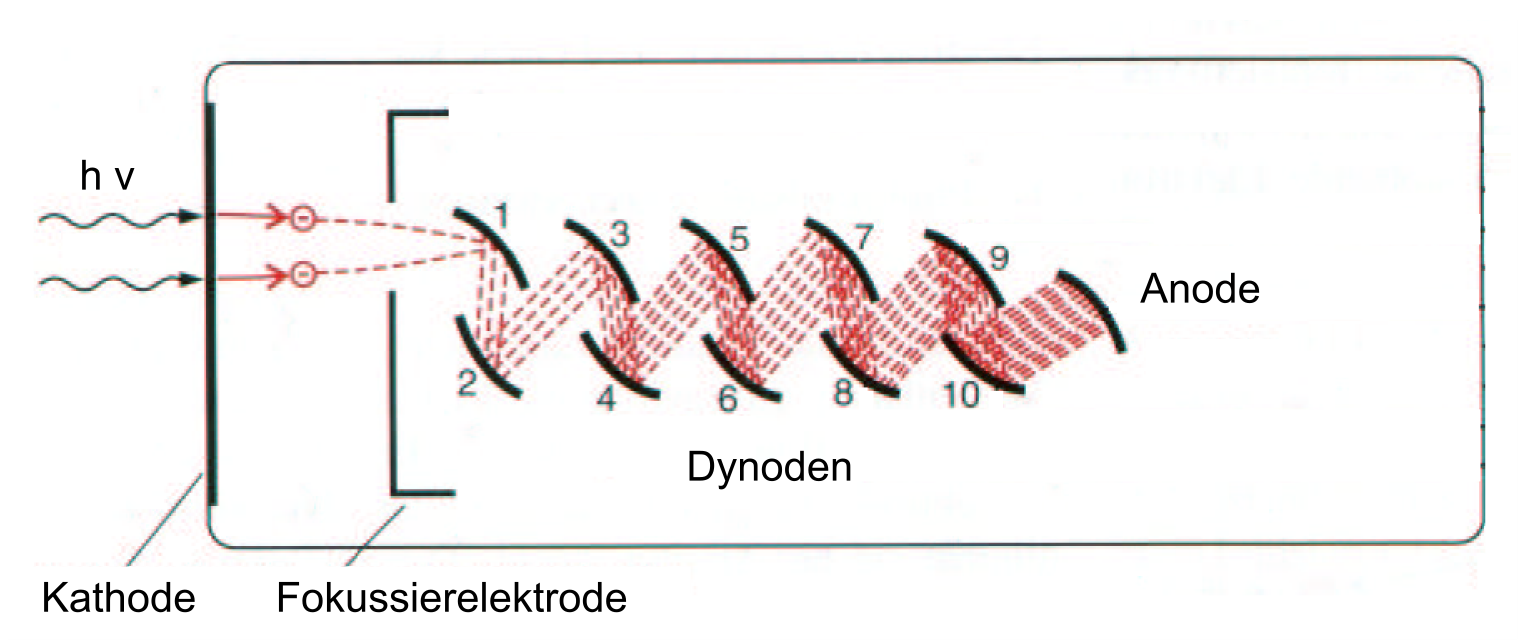
\includegraphics[width=0.55\textwidth]{grafiken/photo}
  \caption[Photomultiplier]{Prinzip eines Photomultipliers~\cite{dem3},
  bearbeitet}
  \label{fig:photo}
\end{figure}

\section{Versuchsaufbau}

\section{Versuchsdurchf�hrung und Auswertung}
\newcommand{\plot}[1]{
  \begin{tikzpicture}
    \begin{axis}[xlabel={$\text{Winkel}/^\circ$},
                 ylabel=Z�hlrate,
                 xtick={0, 30, ..., 330}]
      \addplot+[only marks, mark=.]
        plot[error bars/.cd, x dir=both, x fixed=1, y dir=both, y fixed=100]
          function {'data/#1.txt' u 1:2};
    \end{axis}
  \end{tikzpicture}
}

\subsection{Untergrundmessung}


\section{Zusammenfassung}


\begin{appendix}
  \Literatur{quellen}

\end{appendix}
\end{document}
